\documentclass{article}
\usepackage{graphicx}
\usepackage{float}
\usepackage{svg}
\usepackage{amsmath}
\usepackage{amsthm}
\usepackage{caption}

\usepackage{mathtools}
\DeclarePairedDelimiter\ceil{\lceil}{\rceil}

\def \scalingfactor{.8}

\begin{document}

\title{Benchmarking Fermi Microarchitecture}
\author{Paolo Ienne, Andrea Miele\and Ewaida Moshen, Cl\'{e}ment Humbert, Tristan Overney}
\date{\today}
\maketitle

\section{Goals}
	The goals of this benchmarking is to expose the Fermi microarchitecture details
    as implemented in Nvidia Fermi cards (pipeline length, instructions latency,
    scheduling patterns, etc.) in order to know what can and cannot be changed
    to create an integer computation oriented device.

\section{Methods}
	To achieve the aforementioned goals, a serie of specially crafted CUDA kernels
	were used. These usually contain large batches of dependent instructions that were 
	timed with the assistance of the \texttt{clock64()} function offered by the CUDA API.

	The benchmark programs have been ran on a machine equipped with an Nvidia
    GeForce GTX 580 GPU.

\section{Terminology}
    Before diving into the experiments and their results here's a quick-start
    guide to Nvidia's Fermi architecture and its vocabulary:

    \subsection{Streaming Multiprocessors}
    The largest building block inside the Fermi architecture is the 
    \emph{Streaming multiprocessor} (Figure ~\ref{fig:SM} on page 
    ~\pageref{fig:SM}) abbreviated SM in this report. Fermi cards are equipped
    with 16 of these SMs.
    \begin{figure}[H]
    \centering
        \includesvg[width=\scalingfactor\linewidth]{FermiSM}
        \caption{Fermi's streaming multiprocessor schematic representation}
        \label{fig:SM}
    \end{figure}

    Each SM is composed of the following computation blocks:
    \begin{itemize}
        \item 32 CUDA cores in two groups of 16,
        \item 16 load/store units (LD/ST on the figure)
        \item 4 Special Functions Units (SFUs) dedicated to more complex
              arithmetic functions such as sines and logarithms.
    \end{itemize}
    
    As the SFU is dedicated to floating-point operations it's already an area
    that can be reused for integer computation components, thus it's not part
    of the following research. The focus of the experiments are the CUDA cores.

    \subsection{CUDA Cores}
    Figure~\ref{fig:CUDACore} is the representation of what a CUDA core is,
    according to Nvidia.
    
    \begin{figure}[H]
    \centering
        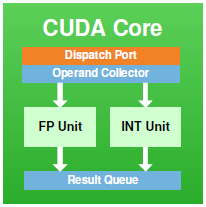
\includegraphics{pictures/CUDACore}
        \caption{Schematic representation of Nvidia's CUDA Core}
        \label{fig:CUDACore}
    \end{figure}
    
    From figure~\ref{fig:CUDACore} the notion of twice 16 cores can be
    adjusted to twice 16 integers ALUs and 16 simple-precision floating-point
    ALUs.

    \subsection{Basics of Fermi's scheduling}
        \subsubsection{Grids and blocks} 
        A cuda kernel (that is: a section of code that will run on the GPU) is
        launched with two parameters: a grid size and a block size. The grid 
        size is used to determine the number of SM on which the code will run.
        The block size determines how many threads will run the code inside each
        SM. As we're interested in the properties of single SMs or even, single
        cores, every benchmarking experiment was done using a grid size of one.

        \subsubsection{Warps}
        The second important scheduling unit is the warp. A warp consists
        of 32 threads. Each scheduling cycle, the scheduler selects two
        warps, for each of these it schedules 16 threads (making it 32
        threads coming from two warps).

\section{Pipeline properties}
	This section contains the results obtained through the previously described
	methods using large batches of integer multiplications.

	\subsection{Benchmark running times against number of threads}
	\label{par:pipeline_exp}
	\subsubsection{Description of the experiment}
	The following experiment is trying to outline the relation between the running
    times of the benchmark program and the number of threads running parallely in
    a single block (the threads reside on one SM).
	\subsubsection{Expectations}
    The running times are expected to be slightly higher for the integer
    multiplications but to deteriorate in a similar fashion (begin to deteriorate
    at the same point, at the same rate) due to each core being equipped with
    integer and single-precision floating-point ALUs.
    
	\subsubsection{Results and analysis}
    \begin{figure}[h]
    	\centering
		\vspace{-20pt}
        % TODO: replace with graphic containing both INT and FP results
	    \includegraphics[width=\scalingfactor\linewidth]{"graphics/running_times"}
		\vspace{-15pt}
        \caption{Running times of benchmark (in cycles) against number of threads}
    \end{figure}
	\pagebreak
    
    \subsubsection{Results}
    The results are against the expectations as it's easy to see the integer
    multiplication times starting to grow at 257 threads in the block against
    513 for the simple-precision floating-point multiplications.
    
    %not at the right place, there should be a section about FP benchmark.
    Seeing as the running time is constant up to 512 threads running and that we have 32 cores avaliable it has been assumed that the pipeline depth for the FP multiplication is 16 ($512/32 = 16$). Which seems to correlate with the latency of the FP multiplication.
    \ref{fig:fp_prediction_tabel} represent the analysis that has been drawn when 512 threads are running, $C_1$ to $C_{32}$ are the core of the single SM on which the experiment has been run. (1 to 16 is the first core group and 17 to 32 is the second one.) $t_{j,k}$ is the thread nb $k$ of the warp $j$. 
        \begin{figure}[h]
      \centering
       \begin{tabular}{ | r || c | c | c | c | c | c | c | }
    	    \hline
    	    time since begining & $C_1$ & $C_2$ & ... & $C_{16}$ & $C_{17}$ & ... & $C_{32}$ \\ \hline  \hline
    	   1 & $t_{1,1}$ & $t_{1,2}$ & ... & $t_{1,16}$ & $t_{2, 1}$ & ... & $t_{2, 16}$ \\ \hline 
    	   2 & $t_{1,17}$ & $t_{1,18}$ & ... & $t_{1,32}$ & $t_{2, 17}$ & ... & $t_{2, 32}$ \\ \hline
    	   ... & ... & ... & ... & ... & ... & ... & ... \\ \hline
    	   16 & $t_{15,17}$ & $t_{15,18}$ & ... & $t_{15,32}$ & $t_{16,17}$ & ... & $t_{16, 32}$ \\ \hline
    	   17 & $t_{1,1}$ & $t_{1,2}$ & ... & $t_{1,16}$ & $t_{2, 1}$ & ... & $t_{2, 16}$ \\ \hline
  	\end{tabular}
  	\captionsetup{justification=centering}
  	\caption{$C_1$ to $C_{32}$ are the core of a single SM \newline$t_{j,k}$ is the thread nb $k$ of the warp $j$.}
  	\label{fig:fp_prediction_tabel}
   \end{figure}

	% better phrasing needed :)
    To understand these deteriorations points the next experiment has been designed.

\section{Mixing single-precision floating-points and integer multiplication}
	\subsection{The experiment}
	Information has been found which was implying that the number of integer multiplication
    able to run parallely on an SM was only half the number single-precision floating-point
    multiplication. Leading to the conclusion that only one of the two 16 cores group of an
    SM was equipped with integer. The following experiments issue integer multiplication in
    parallel of floating-point operations to confirm this hypothesis.
	\subsection{Benchmark running times, 1 single-precision floating-points for 1 integer multiplication}
	If indeed only 1 out of 2 cores group can run integer multiplication then
    adding the same amount of floating-point multiplications as there were integer
    multiplications should not increase the total time spent executing the benchmark 
    program as the single-precision floating-point multiplication can
    be ran on the other core group (the one that does not possess integer multiplication).
	
	One million multiplication of each kind has been ran on 1 to 1024 threads to
    see if the results were comparable to the graph were there was only integer multiplication.
	\begin{figure}[h]
		\centering
		\vspace{-20pt}
    			\includegraphics[width=\scalingfactor\linewidth]{"graphics/running_times_ratio11"}
		\vspace{-15pt}
		\caption{Integer/Floating point multiplication ratio: 1}
	\end{figure}
	\pagebreak

	\subsection{Benchmark running times with mixed single-precision floating-point and integer multiplications}
	\begin{figure}[h]
		\centering
		\vspace{-20pt}
        \includegraphics[width=\scalingfactor\linewidth]{"graphics/running_times_mixed"}
		\vspace{-15pt}
        \caption{Running times of benchmarks with a mix of single-precision floating-points and integers multiplications}
    \end{figure}

    \subsection{Results}
    The running times appear to be bound by those of the integer multiplication but is no higher than
    when only integer multiplications are ran, this confirms the hypothesis that only 16 of the 32
    CUDA core are equipped with integer ALUs.

\section{Understanding pipeline length and performance deterioration}
    \subsection{The experiment}
    With the results of \ref{par:pipeline_exp} in mind, it's clear that the core's pipelines
    are of fixed size. The objective of the following experiment is to determine the cost of
    the loop used in the benchmarks to adjust the running times found and match them with
    the hypothesis about pipeline length and scheduling. 
	\subsubsection{Expectations}
	As seen in \ref{par:pipeline_exp} the cost simple-precision floating-point
    operations goes up at 512 threads. This would imply that every pipeline of
    the SM is perfectly filled with 512 threads. Dividing 512 threads by within
    the 32 cores gives a pipeline length of 16. In addition, the cost increase
    is suspected to be 1/8 of the base cost as the scheduling is expected to be
    something like described in the following schematic:
    % TODO INCLUDE SCHEDULING SCHEMATIC

    The 1/8 can be derived from the following formula:
    \[ \cfrac{t_{513threads} - t_{512threads}}{t_{512threads}} \]
    The latency of an instruction is equal to the pipeline length, plus 1/16 of
    it for every additional warp after the $16^{th}$. So the latency l of an 
    operation is $L + max(0, \ceil{\cfrac{N}{32} -16})$ and to get the total
    running time of a benchmark, this latency must be added as a constant to
    represent the time the last instruction takes to get through the pipeline.

    The expansion of the previous formula gives:
    \[ \cfrac{(16\cdot l_{512} + l_{513} + l_{513}) - (16\cdot l_{512} + l_{512})}{16\cdot l_{512} + l_{512}} \]
    Which, with numerical values and simplifcations is:
    \[ \cfrac{(16\cdot 17 + 2\cdot 17) - (16^2 + 16)}{16^2 + 16} = \cfrac{1}{8}\] 

    Thus, the outcome expected is that once the loop cost is removed from the 
    times obtained in \ref{par_pipeline_exp} the remaining time is 16 millions
    which is 16 cycles per operation, fitting the 16-stages pipeline hypothesis.
    The expected difference in running time after adjustments is 2 millions cycles,
    1/8 of 16 millions.

	\subsubsection{Results and analysis}
    Running a benchmark containing 10 loops of 100000 operations and a benchmark
    of 1000 loops containing 1000 operations yields a difference in running time of
    around 10000 cycles ($\pm$ 800). This leads to a cost of $\sim$ 10 cycles per
    loop iteration. ($t_{1000loops} - t_{10loops} = 10000 \implies t_{990loops} = 10000
    \implies t_{1loop} = 10$)
    
	This means that each warp will run 10 cycles for each loop iteration. Thus the 
    adjusted running times can be computed as follow:
    \[ t_{adj} = t - \ceil{\cfrac{N}{32}}\cdot 10 \cdot n_{iter} \]
    with t, the unadjusted time, $\ceil{\cfrac{N}{32}}$ the number of warps and 
    $n_{iter}$ the number of loop iterations

    Applying the adjustments to the empirical values %TODO 

\section{Results}
    \subsection{Pipeline structure}
    As seen during the experiments, the CUDA core's pipeline appears to be a
    rigid, 16 steps pipeline. The fact that integer multiplication and 
    simple-precision floating-point multiplication both take the same amount
    of time (on a machine that's supposed to be a floating-point calculation
    optimized device) until the pipelines are filled suggests a simple,
    no-dependency-check, scheduler that fires up new instructions every 16 cycles.

    It also appears rather clearly that, while 32 cores per SM are advertised by
    Nvidia, only 16 are equipped with integer ALUs; allowing only 16 integer
    operations to be scheduled every 18 cycles.
    
    \subsection{Prospects}
    From the previous constatations the following ideas are expected to drastically
    improve the integer computation performances while maintaining a stable (if not
    lower) cost in transistors:
    \begin{itemize}
        \item If any instruction is to be added (e.g.: Montgomery's multiplication, larger integer multiplication) these can take up to 18 cycles without having to modify any aspect of the scheduler.
        \item A large amount of integer computation power can be added at low-cost as a whole 16-cores group can be totally replaced by cores dedicated to integer arithmetic.
    \end{itemize}
\section{Additionnal graphics and tables}
	\subsection{Integer multiplication: 1024 threads starting times}
    \begin{figure}[h]
    		\centering
		\vspace{-20pt}
	    	\includegraphics[width=\scalingfactor\linewidth]{"graphics/starting_times_ratio31"}
	    	\vspace{-15pt}
	    	\caption{Order in which thread batches are started}
    \end{figure}

    \subsection{Graphics intersteps data}
    The following tables describe the steps between running times in the graphics presented previously. Analysing them may allow to deduce properties of: 
    \begin{itemize} 
        \item the cores' pipelines, if it represents the delay between dependencies checks;
        \item the scheduling mechanism, if it represents the delaying of threads operations in favor of the launch of other threads.
    \end{itemize}
    \centering
    \begin{tabular}{ccc}
\# & Time delta & Ratio of base execution time\\
1 & 1992038 & 0.110518 \\
2 & 2972214 & 0.164899 \\
3 & 1012084 & 0.056151 \\
4 & 2577818 & 0.143018 \\
5 & 1422160 & 0.078902 \\
6 & 2256334 & 0.125182 \\
7 & 1743568 & 0.096733 \\
8 & 2016076 & 0.111852 \\
9 & 1984078 & 0.110077 \\
10 & 2024116 & 0.112298 \\
11 & 1978718 & 0.109779 \\
12 & 2943966 & 0.163331 \\
13 & 1065326 & 0.059104 \\
14 & 2011174 & 0.111580 \\
15 & 1982664 & 0.109998 \\
16 & 2537828 & 0.140799 \\
17 & 1468682 & 0.081483 \\
18 & 2005218 & 0.111250 \\
19 & 1985786 & 0.110172 \\
20 & 2256680 & 0.125201 \\
21 & 1750700 & 0.097129 \\
22 & 2007560 & 0.111380 \\
23 & 1985942 & 0.110180 \\
\end{tabular}

    \begin{table}
\centering
\begin{tabular}{rcc}
\# & Time delta & Ratio of base execution time\\
\hline
1 & 2147856 & 0.119163 \\
2 & 1934380 & 0.107320 \\
3 & 1997060 & 0.110797 \\
4 & 2026158 & 0.112411 \\
5 & 2009622 & 0.111494 \\
6 & 2007910 & 0.111399 \\
7 & 2018118 & 0.111965 \\
\end{tabular}
\caption{Intersteps between single-precision floating-point multiplications benchmarking}
\end{table}

    \pagebreak
    


\end{document}
